%Ich bin ein TeX Dokument
\documentclass{scrartcl} % KOMA-Script Dokumentenklasse Article
% Warnung, falls noch einmal kompiliert werden muss
\usepackage[aux]{rerunfilecheck}
% Paket für Schriftarteinstellung, muss immer geladen werden
\usepackage{fontspec}
% Deutsche Spracheinstellungen, wichtig z. B. für korrekte Trennung
\usepackage[ngerman]{babel}
% mehr Pakete hier
\usepackage{amsmath}
\usepackage{amssymb}
\usepackage{mathtools}
%ISO Normen benutzen
\usepackage[
math-style=ISO,
bold-style=ISO,
sans-style=italic,
nabla=upright,
partial=upright,
]{unicode-math}
%Für korrekte Zahlen mit Einheiten
\usepackage[
locale=DE,
separate-uncertainty=true,
per-mode=symbol-or-fraction,
]{siunitx}
% Unterstützung für Links und PDF Metadaten
\usepackage[unicode]{hyperref}
\usepackage{bookmark}
\usepackage{pdfpages}
% Einstellungen hier, z.B. Fonts
\setmathfont{Latin Modern Math}
\begin{document}
\title{Titel}
\author{Henry Krämerkämper \and Christopher Breitfeld}
\date{29.10.2020}
\maketitle
\newpage
\tableofcontents
\newpage
\section{Einleitung}
Ein Anfang
\section{Aufgabenteil a)}
  Man stelle die gemessenen Temperaturverläufe in einem geeigneten Diagramm dar. \\
  \\
  Im folgenden Diagramm werden die Verläufe der Temperaturen T1 und T2 in Abhängigkeit der Zeit aufgetragen.
  Alle Werte wurden in SI-Einheiten konvertiert.
  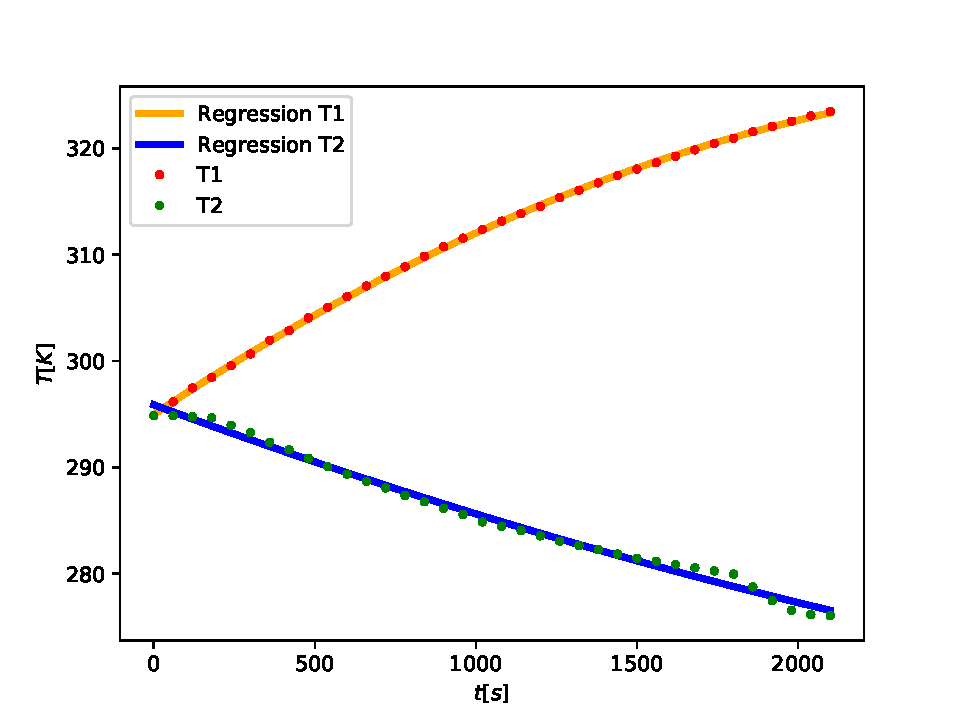
\includepdf{Temperaturverlaeufe.pdf}
\end{document}
